\chapter{Results}
\label{ch:results}

Accuracy of a machine learning model is defined as the number of predictions the model got right, in the case of this classification problem this is predicting the number of booked and cancelled customers. I the case of this prb





\begin{itemize}
\item define accuracy
\item define AUC
\item define F1 score
\item define precision score
\item accuracy overpowered by the amount of booked, if you just look for the high accuracy because of the biased it shows which is the best at showing who's going to book when i want to see who's not going to book
\item talk about probably of cancellation
\end{itemize}


\section{XGboost}



\begin{figure}[hbt!]
 %\centering
 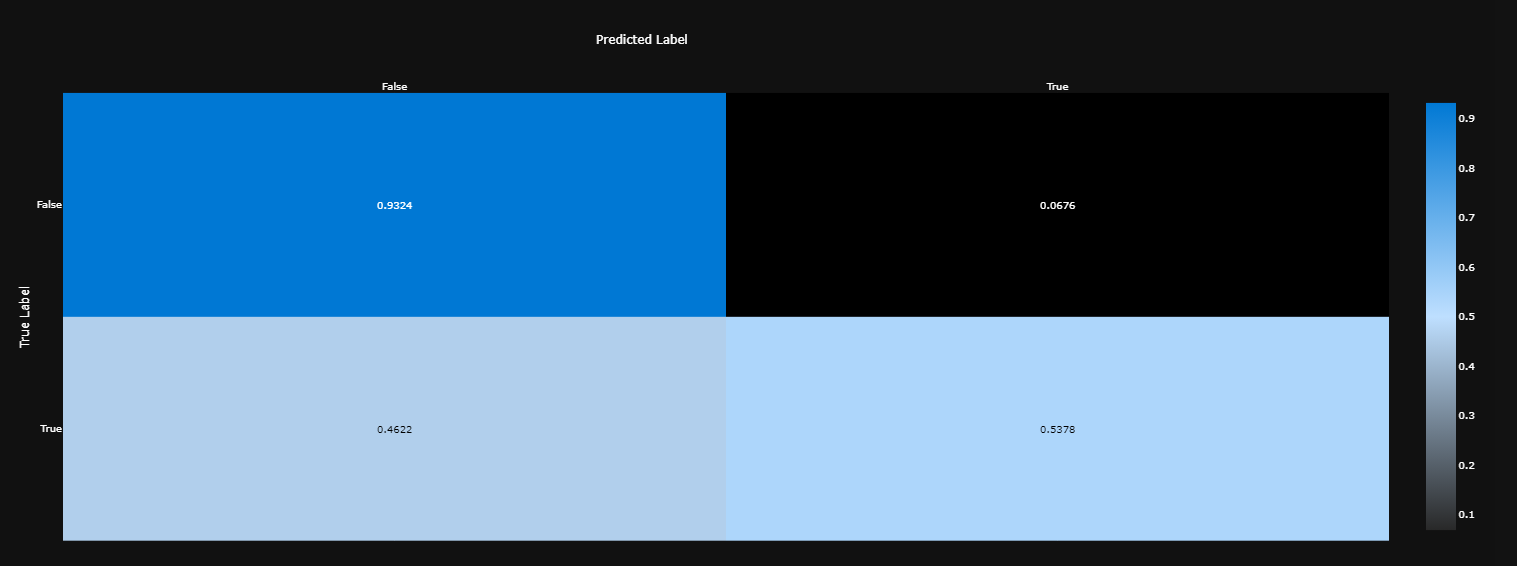
\includegraphics[width=10cm]{figures/azure_ml_confusion_matrix_xg.png}
 \caption{In the field of machine learning and specifically the problem of statistical classification, a confusion matrix, also known as an error matrix, is a specific table layout that allows visualization of the performance of an algorithm, typically a supervised}
\end{figure}

\begin{figure}[hbt!]
 %\centering
 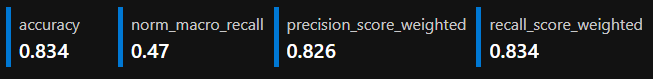
\includegraphics[width=10cm]{figures/xg_boost_scores.png}
 \caption{Scores show high values since it is correctly predicting booked and this overpowers the results as booked makes up 75 percent. meaning a accuracy of 75 would be achieved by predicting everything as booked }
\end{figure}

\begin{itemize}
\item show the accuracy was better with 83
\item the confusion matrix shows that it was worse with more false negatives - cases where I predicated they would book buy they cancelled
\item this was run with no hyperparameter tuning
\item cross validation was used
\end{itemize}



\section{AUTO ML}

\begin{itemize}
\item this is where I did hyperparmater tuning testing X number of different model iterations 
\item with a Target value set to norm macro recall \textbf{explain what this is}
\end{itemize}



\begin{itemize}
\item start with confusion matrix
\item talk about true trues - this is the number of booking cancellations I was able to predict correctly 
\end{itemize}

\begin{figure}[hbt!]
 %\centering
 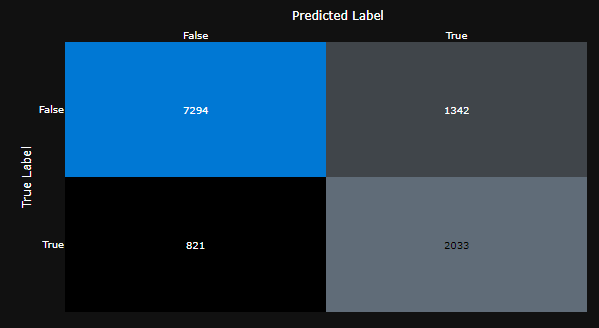
\includegraphics[width=10cm]{figures/azure_ml_confusion_matrix.png}
 \caption{In the field of machine learning and specifically the problem of statistical classification, a confusion matrix, also known as an error matrix, is a specific table layout that allows visualization of the performance of an algorithm, typically a supervised}
\end{figure}

Figure 4.1 shows I was able to predict 2033 True True values with 821 False positives this is a ratio of 0.71 to 0.28

\begin{figure}[hbt!]
 %\centering
 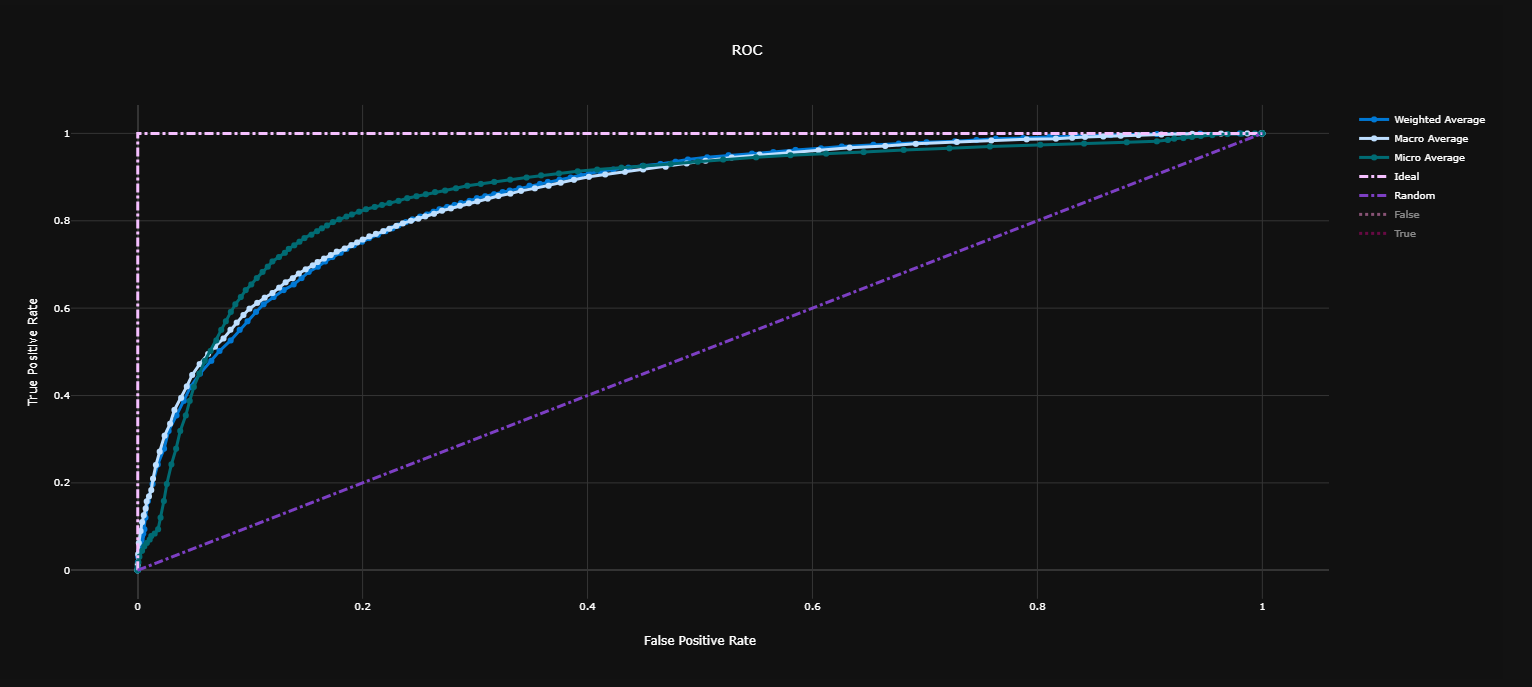
\includegraphics[width=10cm]{figures/azure_ml_roc.png}
 \caption{}
\end{figure}

\begin{itemize}
\item talk about the precision
\item talk about the recall 
\item talk about the F1 score
\item for all of these compare expected with actual
\item how many more values are predicted correctly when comparing the 2 methods
\end{itemize}
